\documentclass[10pt,journal,letterpaper,compsoc]{IEEEtran} 

\usepackage{times}
\usepackage{epsfig}
\usepackage{graphicx}
\usepackage{amsmath}
\usepackage{amsfonts}
\usepackage{amscd}
\usepackage{amssymb}
\usepackage{subfigure}
\usepackage{pdfsync}
\usepackage{helvet}
\usepackage{url}
\usepackage{color}

% Include other packages here, before hyperref.
\usepackage{mydefs}
\usepackage{algorithm}
\usepackage{algorithmic}

\usepackage{multirow}
\usepackage{pict2e}
\usepackage{slashbox}


% \usepackage[small]{caption}

\newcommand{\subj}{\textup{subj to}}

\newcommand{\jw}[1]{{\bf \textcolor{blue}{John: #1}}}
%\newcommand{\aw}[1]{\bf \color{greem} Drew: #1}
%\newcommand{\ym}[1]{\bf \color{red}{ Yi: #1}}

\newcommand{\zz}[1]{{\bf \textcolor{red}{Zihan: #1}}}

\begin{document}
%
% paper title
\title{Towards a Practical Face Recognition System: \\ Robust Alignment and
Illumination by Sparse Representation\\
(Supplementary Materials)}
%
% author names and IEEE memberships
% note positions of commas and nonbreaking spaces ( ~ ) LaTeX will not break
% a structure at a ~ so this keeps an author's name from being broken across
% two lines.
% use \thanks{} to gain access to the first footnote area
% a separate \thanks must be used for each paragraph as LaTeX2e's \thanks
% was not built to handle multiple paragraphs
\author{Andrew~Wagner,~\IEEEmembership{Student~Member,~IEEE,}
        John~Wright,~\IEEEmembership{Member,~IEEE,}
        Arvind~Ganesh,~\IEEEmembership{Student~Member,~IEEE,}
        Zihan~Zhou,~\IEEEmembership{Student~Member,~IEEE,}
        Hossein~Mobahi,
        and~Yi~Ma,~\IEEEmembership{Senior~Member,~IEEE}% <-this % stops a space
\thanks{A. Wagner, A. Ganesh, Z. Zhou, and Y. Ma are with the Dept. of Electrical and Computer Engineering at the University of Illinois at Urbana-Champaign. H. Mobahi is with the Computer Science Dept. at the University of Illinois at Urbana-Champaign.  J. Wright and Y. Ma are with Microsoft Research Asia.  Corresponding author: Andrew Wagner, awagner@illinois.edu, 1308 W. Main st. Urbana, IL 61801, (312) 343-1380.}}% <-this % stops a space

% The paper headers
%\markboth{Journal of \LaTeX\ Class Files,~Vol.~1, No.~8,~August~2002}{Shell \MakeLowercase{\textit{et al.}}: Bare Demo of IEEEtran.cls for Journals}
% The only time the second header will appear is for the odd numbered pages
% after the title page when using the twoside option.

\maketitle

\IEEEdisplaynotcompsoctitleabstractindextext
\vspace{-9mm} % HACK

\IEEEpeerreviewmaketitle

%%%%%%%%% BODY TEXT
\section{L1 Minimization via Augmented Lagrange Multiplier}

\PARstart{I}{n} these supplementary materials we discuss the computational issues related to
the implementation of Algorithm~\ref{alg:deformable-src}, which is
repeated here for convenience. It is
not hard to see that its computational complexity is dominated
by the two steps where the $\ell^1$-norm minimization problems
are solved; namely Step 6 for iterative registration, and Step
14 for global sparse representation.
Fortunately, many fast algorithms for solving these problems have been proposed over the
past ten years. We refer the interested reader to \cite{YangA2010-pp} for a more comprehensive survey of the developments in this area.
That work suggests that \emph{Augmented Lagrange Multiplier}
(ALM) algorithms \cite{Bertsekas1982} strike a good balance
between scalability and accuracy: as first order methods, they
require only lightweight vector operations and matrix-vector
multiplications at each iteration, making them preferable to
more classical solutions such as interior point methods.
However, compared to other first-order methods, they achieve
higher accuracy with a fixed computational budget.
\begin{algorithm}[thb]
\caption{\bf (Deformable Sparse Recovery and Classification for
Face Recognition)} \label{alg:deformable-src}
\begin{algorithmic}[1]
\begin{small}
\STATE {\bf Input:} Training images $\{A_i \in \Re^{m\times n_i}\}_{i=1}^K$ for $K$ subjects,  a test image
$\y\in\Re^m$ and a deformation group $T$.
\STATE
{\bf for} each subject $i$,
\STATE \hspace{3mm} $\tau^{(0)}
\leftarrow I$.
\STATE \hspace{3mm} {\bf while} not converged $(j=1,2,\ldots)$ {\bf do}
\STATE \hspace{6mm}
$\tilde \y(\tau) \leftarrow \frac{\y \circ \tau}{\|\y \circ
\tau\|_2}$; \;\;\; $J \leftarrow  \frac{\partial}{\partial
\tau} \tilde\y(\tau)  \bigr|_{\tau^{(j)}} $;
%\STATE \hspace{6mm} $(\hat \x, \hat \e, \Delta \tau) \leftarrow \left\{\begin{array}{l} \arg \min_{\x,\e,\Delta \tau} \| \e \|_1 \\  \subj \; \y + J \Delta \tau = A_k \x + \e \end{array}\right.$
\STATE \hspace{6mm} $ \Delta \tau =  \arg\min \; \| \e \|_1  \;
\subj \; \tilde \y + J \Delta \tau = A_i \x + \e.$
\STATE
\hspace{6mm} $\tau^{(j+1)} \leftarrow \tau^{(j)} + \Delta
\tau$;
\STATE \hspace{3mm} {\bf end while} \STATE {\bf end} \STATE Keep
the top $S$ candidates $k_1, \ldots, k_S$ with the smallest
residuals $\|\e\|_1$. \STATE Compute an average transformation
$\bar{\tau}$ from $\tau_{k_1}, \tau_{k_2}, \ldots, \tau_{k_S}$.
\STATE Update $\y \leftarrow \y \circ \bar{\tau}$ and $\tau_i
\leftarrow \tau_i \cdot \bar{\tau}^{-1}$ for $i = k_1, \dots,
k_S$. \STATE Set $A \leftarrow \big[ A_{k_1} \circ
\tau_{k_1}^{-1} \mid A_{k_2} \circ \tau_{k_2}^{-1} \mid \dots
\mid A_{k_S} \circ \tau_{k_S}^{-1} \big]$. \STATE Solve the
$\ell^1$-minimization problem: \hspace{2mm}
$\hat{\x} = \arg \min_{\x, \e} \| \x \|_1 + \|\e\|_1 \;\; \subj \;\; \y = A \x + \e.$
\STATE Compute residuals $r_i(\y) = \| {\y} - {A}_i \, \delta_i(\hat{\x}) \|_2$ for $i = k_1, \dots, k_S$.
\STATE {\bf Output:} $\mbox{identity}(\y) = \arg\min_i r_i(\y)$.
\end{small}
\end{algorithmic}
\end{algorithm}
%\vspace{-4mm}


We use Step 14 as an example to illustrate the ALM
method, since solving Step 6 is very similar. Recall that in
Step 14 the problem we are interested in is:
\begin{equation}
\min_{\x, \e} \| \x \|_1 + \|\e\|_1 \quad \subj \quad \y =
A \x + \e.
\end{equation}
Its corresponding augmented Lagrangian function is
\begin{equation}
L_\mu (\x,\e,\blamda) = \|\x\|_1 + \|\e\|_1 + \langle \blamda, \y-A\x - \e \rangle + \frac{\mu}{2} \|\y - A\x - \e\|_2^2,
\end{equation}
where $\blamda$ is the Lagrange multiplier and $\mu > 0$ is a
penalty parameter. The ALM method seeks a saddlepoint of $L_\mu
(\x,\e,\blamda)$ by alternating between optimizing with respect
to the primal variables $\x, \e$ and updating the dual variable
$\blamda$, with the other fixed, as follows:
\begin{equation}
\left \{
\begin{array}{lll}
(\x_{k+1},\e_{k+1})  =  \arg\min_{(\x,\e)} \, L_{\mu} (\x,\e,\blamda_k),\\
\blamda_{k+1}  =  \blamda_k + \mu (\y - A\x_{k+1} - \e_{k+1}). \\
\end{array}
\right .
\label{eq:alm}
\end{equation}
Although updating $\blamda$ is trivial,
minimizing $L_{\mu} (\x,\e,\blamda_k)$ with respect to both
$\x$ and $\e$ could still be costly. To further reduce the
complexity of the problem, we adopt an approach used in
\cite{YangJ2009-pp}, called \emph{alternating direction
method of multipliers} (ADM) \cite{Glowinski1975-TR}, which alternates between minimizing $L_{\mu} (\x,\e,\blamda_k)$
over $\x$ (with $\e$ fixed) and over $\e$ (with $\x$ fixed). After solving these two subproblems, the Lagrange multiplier $\blamda$ is updated, yielding an iteration of the form:
\begin{equation}
\left \{
\begin{array}{lll}
\e_{k+1}  =  \arg\min_{\e} \, L_{\mu} (\x_k,\e,\blamda_k),\\
\x_{k+1}  =  \arg\min_{\x} \, L_{\mu} (\x,\e_{k+1},\blamda_k),\\
\blamda_{k+1}  =  \blamda_k + \mu (\y - A\x_{k+1} - \e_{k+1}). \\
\end{array}
\right .
\label{eq:adm}
\end{equation}
As the objective function is convex and alternation is between two
terms, this procedure is guaranteed to converge to a global optimum (see \cite{YangJ2009-pp} and references therein).

In order to discuss the solution to the above subproblems, we
need to define the following soft-thresholding operator for a
vector $\x$ and a scalar $\alpha \geq 0$:
\begin{equation}
\mathcal{T}(\x,\alpha) = \textup{sign}(\x)\cdot \max \{|\x| - \alpha, 0\},
\end{equation}
where all the operations are performed component-wise. It is
easy to show that the subproblem with respect to $\e$ has a
closed-form solution given by the soft-thresholding operator:
\begin{equation}
\e_{k+1} = \mathcal{T}(\y - A\x_k + \mu^{-1}\blamda_k, \mu^{-1}).
\end{equation}
To solve the subproblem associated with $\x$, we
apply a first-order $\ell^1$-minimization method,
called \emph{fast iterative shrinkage-threshold algorithm}
(FISTA) \cite{BeckA2009}. The main idea of FISTA is to
iteratively minimize a quadratic approximation $Q(\x, \z)$ to
$L_{\mu} (\x,\e_{k+1},\blamda_k)$ around a point $\z$, which is
carefully chosen in order to achieve a good convergence
rate. We summarize the entire ALM
algorithm as Algorithm~\ref{alg:alm}, where $\gamma$ denotes the
largest eigenvalue of the matrix $A^TA$. For the choice of parameter $\mu$, we take the same strategy as
in \cite{YangJ2009-pp} and set $\mu = 2m / \|\y\|_1$.
\begin{algorithm}[t]
\caption{\bf (Augmented Lagrange Multiplier Method for Global
Recognition)}
\begin{algorithmic}[1]
\begin{small}
\STATE {\bf Input:} $\y \in \Re^m$, $A \in \Re^{m \times n}$,
$\x_1 = \mathbf{0}$, $\e_1 = \y$, $\blamda_1 =
\mathbf{0}$.
\WHILE{not converged ($k = 1,2,\ldots$)}
\STATE $\e_{k+1} = \mathcal{T}\left(\y - A\x_k +
\frac{1}{\mu}\blamda_k, \frac{1}{\mu}\right)$;
\STATE $t_1\leftarrow 1$, $\z_1 \leftarrow \x_k$, $\w_1 \leftarrow \x_k$;
\WHILE{not converged ($l = 1,2,\ldots$)}
\STATE $\w_{l+1} \leftarrow \mathcal{T}\left(\z_l +
\frac{1}{\gamma}A^T\left(\y - A\z_l - \e_{k+1} +
\frac{1}{\mu}\blamda_k\right), \frac{1}{\mu\gamma}\right)$;
\STATE $t_{l+1} \leftarrow \frac{1}{2}\left( 1 +
\sqrt{1+4t_l^2}\right)$;
\STATE $\z_{l+1} \leftarrow \w_{l+1} + \frac{t_l - 1}{t_{l+1}}(\w_{l+1} - \w_l)$;
\ENDWHILE
\STATE $\x_{k+1} \leftarrow \w_{l}$,  \; $\blamda_{k+1} \leftarrow \blamda_k + \mu (\y - A\x_{k+1} - \e_{k+1})$;
\ENDWHILE \STATE
{\bf Output:} $\x^* \leftarrow \x_k, \e^* \leftarrow \e_k$.
\end{small}
\end{algorithmic}
\label{alg:alm}
%\vspace{-4mm}
\end{algorithm}

We have selected this algorithm because it strikes the best
balance between speed, accuracy, and scalability for our problem out of
many algorithms that we have tested. We refer the interested reader to
\cite{YangA2010-pp} for a more detailed discussion of competing
approaches.  On a Mac Pro with
Dual-Core 2.66GHz Xeon processors and 4GB memory,
running on our database containing images size $80\times 60$
pixels from 109 subjects under 38 illuminations,
our C implementation of Algorithm~\ref{alg:deformable-src} takes
about 0.60 seconds per subject for alignment and about 2.0
seconds for global recognition. Compared to the highly
customized interior point method used in the conference version
of this paper \cite{Wagner2009-CVPR}, this new algorithm is
only slightly faster for per subject alignment. However, it is
much simpler to implement and it achieves a
\emph{speedup of more than a factor of 10} for global
recognition!

\bibliographystyle{IEEEtran}
\bibliography{faces}

% Biography section
\newcommand{\biospace}{\vspace{-2em}}
\biospace
\begin{IEEEbiography}[{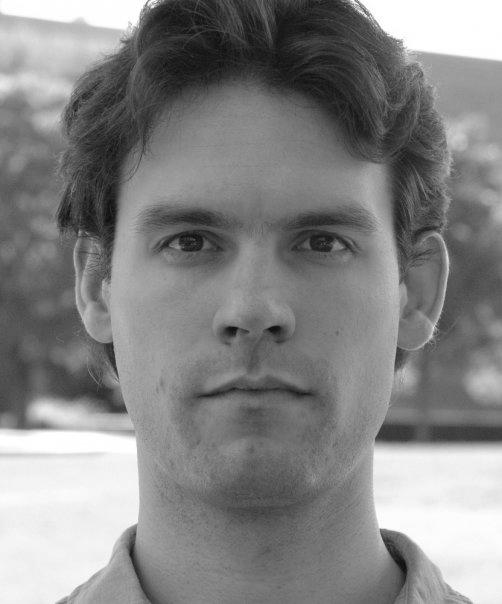
\includegraphics[width=1in,height=1.25in,clip,keepaspectratio]{bios/drew}}]{Andrew Wagner}
received his Bachelor's degree in General Engineering in 2003,
and his Master's degree in Electrical Engineering in 2006, from the University
of Illinois at Urbana-Champaign, where he is currently a Ph.D.
candidate in Electrical \& Computer Engineering.
His research interests include robotics, computer vision, and optimal control.
His recent work focuses on parallel algorithms for sparsity
based face recognition.\end{IEEEbiography}

\biospace
\begin{IEEEbiography}[{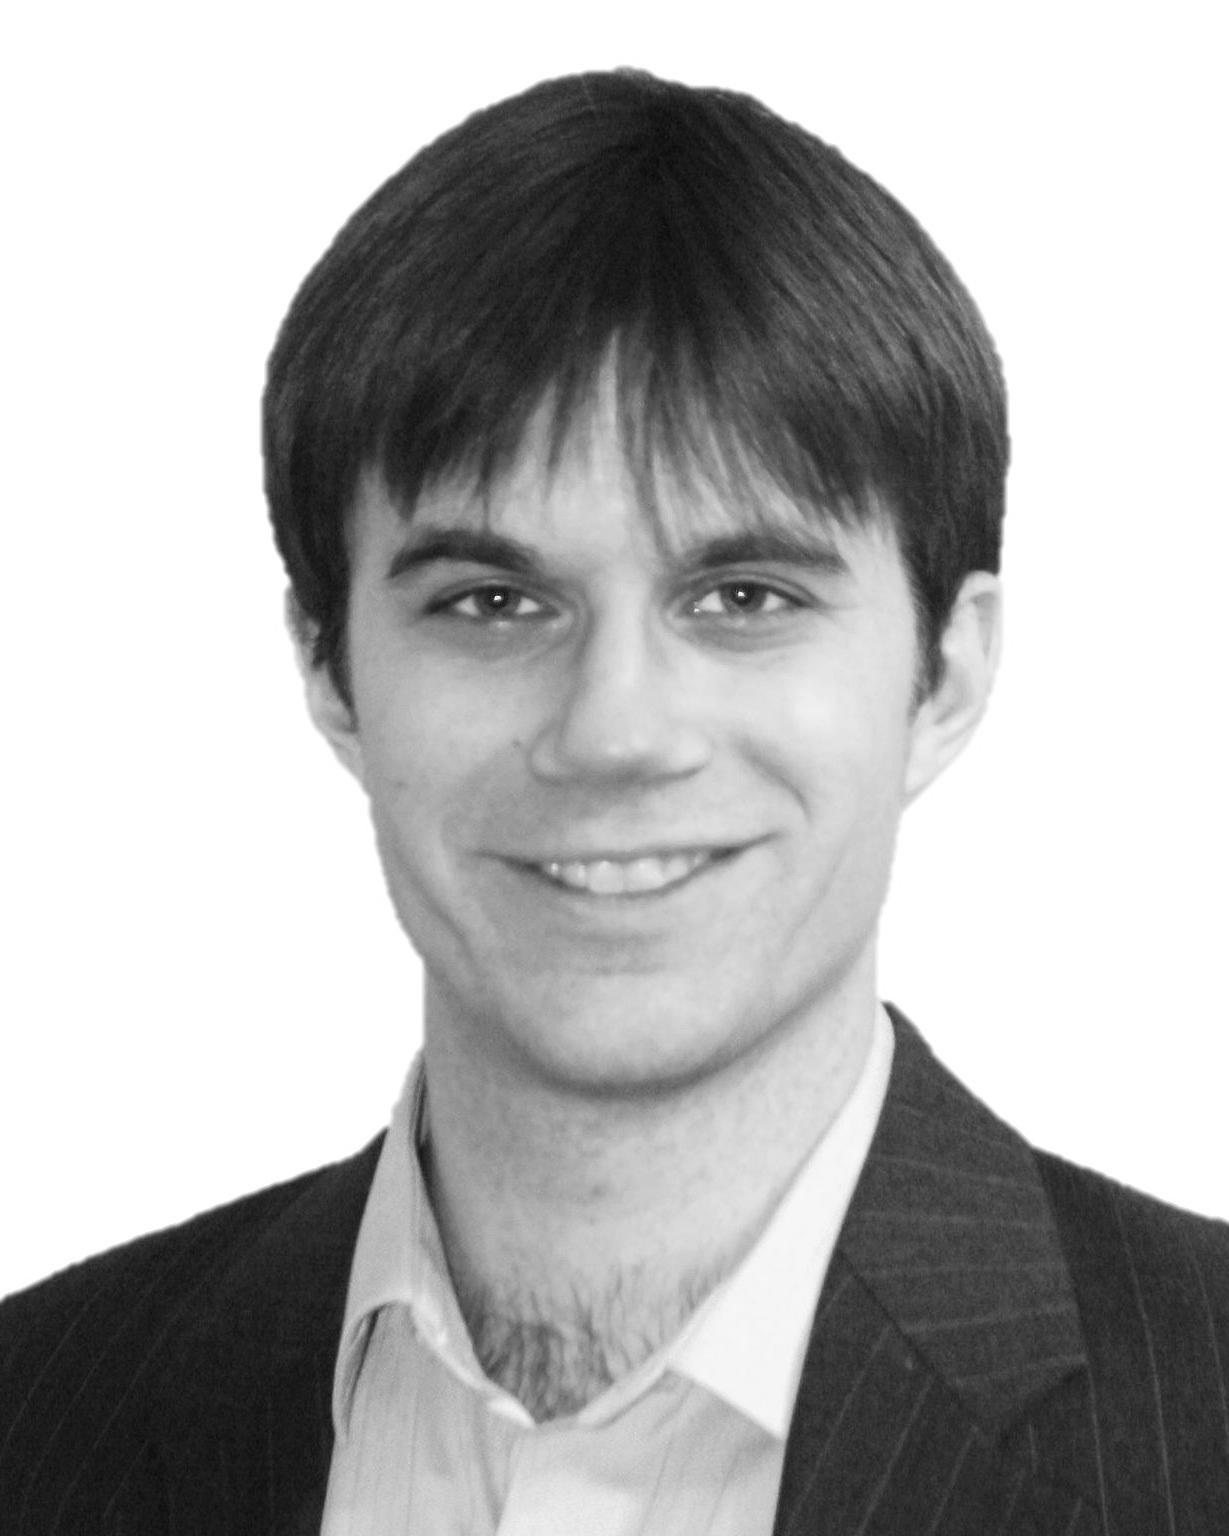
\includegraphics[width=1in,height=1.25in,clip,keepaspectratio]{bios/john}}]{John
Wright} received his PhD in Electrical Engineering from the
University of Illinois at Urbana-Champaign in October 2009. He is currently a
researcher in the Visual Computing group at Microsoft Research Asia.  His
research focuses on developing provably correct and efficient tools for
recovering low-dimensional structure in corrupted high-dimensional datasets.
His work has received a number of awards, including the 2009 Lemelson-Illinois
Prize for Innovation, the 2009 UIUC Martin Award for Excellence in Graduate
Research, a 2008-2010 Microsoft Research Fellowship, a Carver fellowship, and a
UIUC Bronze Tablet award.  \end{IEEEbiography}

\biospace
\begin{IEEEbiography}[{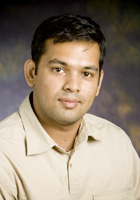
\includegraphics[width=1in,height=1.25in,clip,keepaspectratio]{bios/arvind}}]{Arvind Ganesh}
received his Bachelor's and Master's degrees, both in Electrical
Engineering, from the Indian Institute of Technology, Madras, India in 2006. He
is currently a PhD candidate in the Electrical \& Computer Engineering
Department at the University of Illinois, Urbana-Champaign. His research
interests include compressed sensing, computer vision, and machine learning.
His recent work focuses on low-rank matrix recovery techniques for
batch image alignment and texture rectification.  \end{IEEEbiography}

\biospace
\begin{IEEEbiography}[{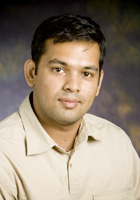
\includegraphics[width=1in,height=1.25in,clip,keepaspectratio]{bios/arvind}}]{Zihan Zhou}
received... {\bf PLACEHOLDER}
\end{IEEEbiography}

\biospace
\begin{IEEEbiography}[{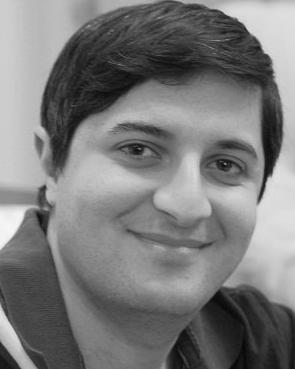
\includegraphics[width=1in,height=1.25in,clip,keepaspectratio]
{bios/hossein}}]{Hossein Mobahi} received his Bachelor's and Master's degrees
in Iran, both in Computer Engineering from Azad University (Tehran-South) in
2003  and University of Tehran in 2005 respectively. He is currently a PhD
candidate in the Computer Science Department at the University of Illinois,
Urbana-Champaign. His research interests include pattern classification,
clustering and optimization.  His recent research focuses on iterative
smoothing for image alignment.  \end{IEEEbiography}

\biospace
\begin{IEEEbiography}[{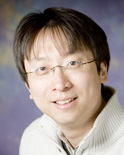
\includegraphics[width=1in,height=1.25in,clip,keepaspectratio]{bios/yi}}]{Yi
Ma} received two Bachelors degree in Automation and Applied Mathematics
from  Tsinghua University, Beijing, China, in 1995. He received an Master
degree in Electrical Engineering and Computer Sciences (EECS) in 1997, a second
Master degree in Mathematics in 2000, and the Ph.D. degree in EECS in 2000, all
from the University of California at Berkeley. He is currently an associate
professor (with tenure) at the Department of Electrical and Computer
Engineering, University of Illinois at Urbana-Champaign, and since January 2009
has also served as research manager for the Visual Computing Group at Microsoft
Research Asia, Beijing, China.  \end{IEEEbiography}
\vfill

% You can push biographies down or up by placing
% a \vfill before or after them. The appropriate
% use of \vfill depends on what kind of text is
% on the last page and whether or not the columns
% are being equalized.


% Can be used to pull up biographies so that the bottom of the last one
% is flush with the other column.
%\enlargethispage{-5in}


\end{document}
